\documentclass[xcolor=dvipsnames]{beamer}
\usepackage[T1]{fontenc}
\usepackage[utf8]{inputenc}
\usepackage[english,slovak]{babel}

\usepackage{amsmath}
\usepackage{amsthm}
\usetheme{Pittsburgh}
\useoutertheme{shadow}

\usepackage{graphicx}
\usepackage{caption}
\usepackage{subcaption}

\usepackage[]{algorithm2e}
\usepackage{listings}
 \setbeamercovered{transparent}
 \usepackage{cuted}
\usepackage[export]{adjustbox}
\usepackage{mathtools}

\usepackage{lipsum}
\usepackage{verbatim}
\usepackage{transparent}
\usepackage{framed}
\usepackage{xcolor}

\newcommand\Wider[2][3em]{%
\makebox[\linewidth][c]{%
  \begin{minipage}{\dimexpr\textwidth+#1\relax}
  \raggedright#2
  \end{minipage}%
  }%
}




\iftrue

\usetheme{Warsaw}

\setbeamercolor{normal text}{fg=white,bg=black!90}
\setbeamercolor{structure}{fg=white}

\setbeamercolor{alerted text}{fg=red!85!black}

\setbeamercolor{item projected}{use=item,fg=black,bg=item.fg!35}

\setbeamercolor*{palette primary}{use=structure,fg=structure.fg}
\setbeamercolor*{palette secondary}{use=structure,fg=structure.fg!95!black}
\setbeamercolor*{palette tertiary}{use=structure,fg=structure.fg!90!black}
\setbeamercolor*{palette quaternary}{use=structure,fg=structure.fg!95!black,bg=black!80}

\setbeamercolor*{framesubtitle}{fg=white}

\setbeamercolor*{block title}{parent=structure,bg=black!60}
\setbeamercolor*{block body}{fg=black,bg=black!10}
\setbeamercolor*{block title alerted}{parent=alerted text,bg=black!15}
\setbeamercolor*{block title example}{parent=example text,bg=black!15}

\fi



%-------------------------------------------------------------------------------------
\title{\color{white} \bf Deep Q networks}
\author{\color{white} Michal CHOVANEC, PhD}


%\setbeamertemplate{footline}[frame number]{}
\setbeamertemplate{navigation symbols}{}


\date[EURP]{}
\begin{document}

{
    \usebackgroundtemplate
    {
        \vbox to \paperheight{\vfil\hbox to \paperwidth{\hfil

        {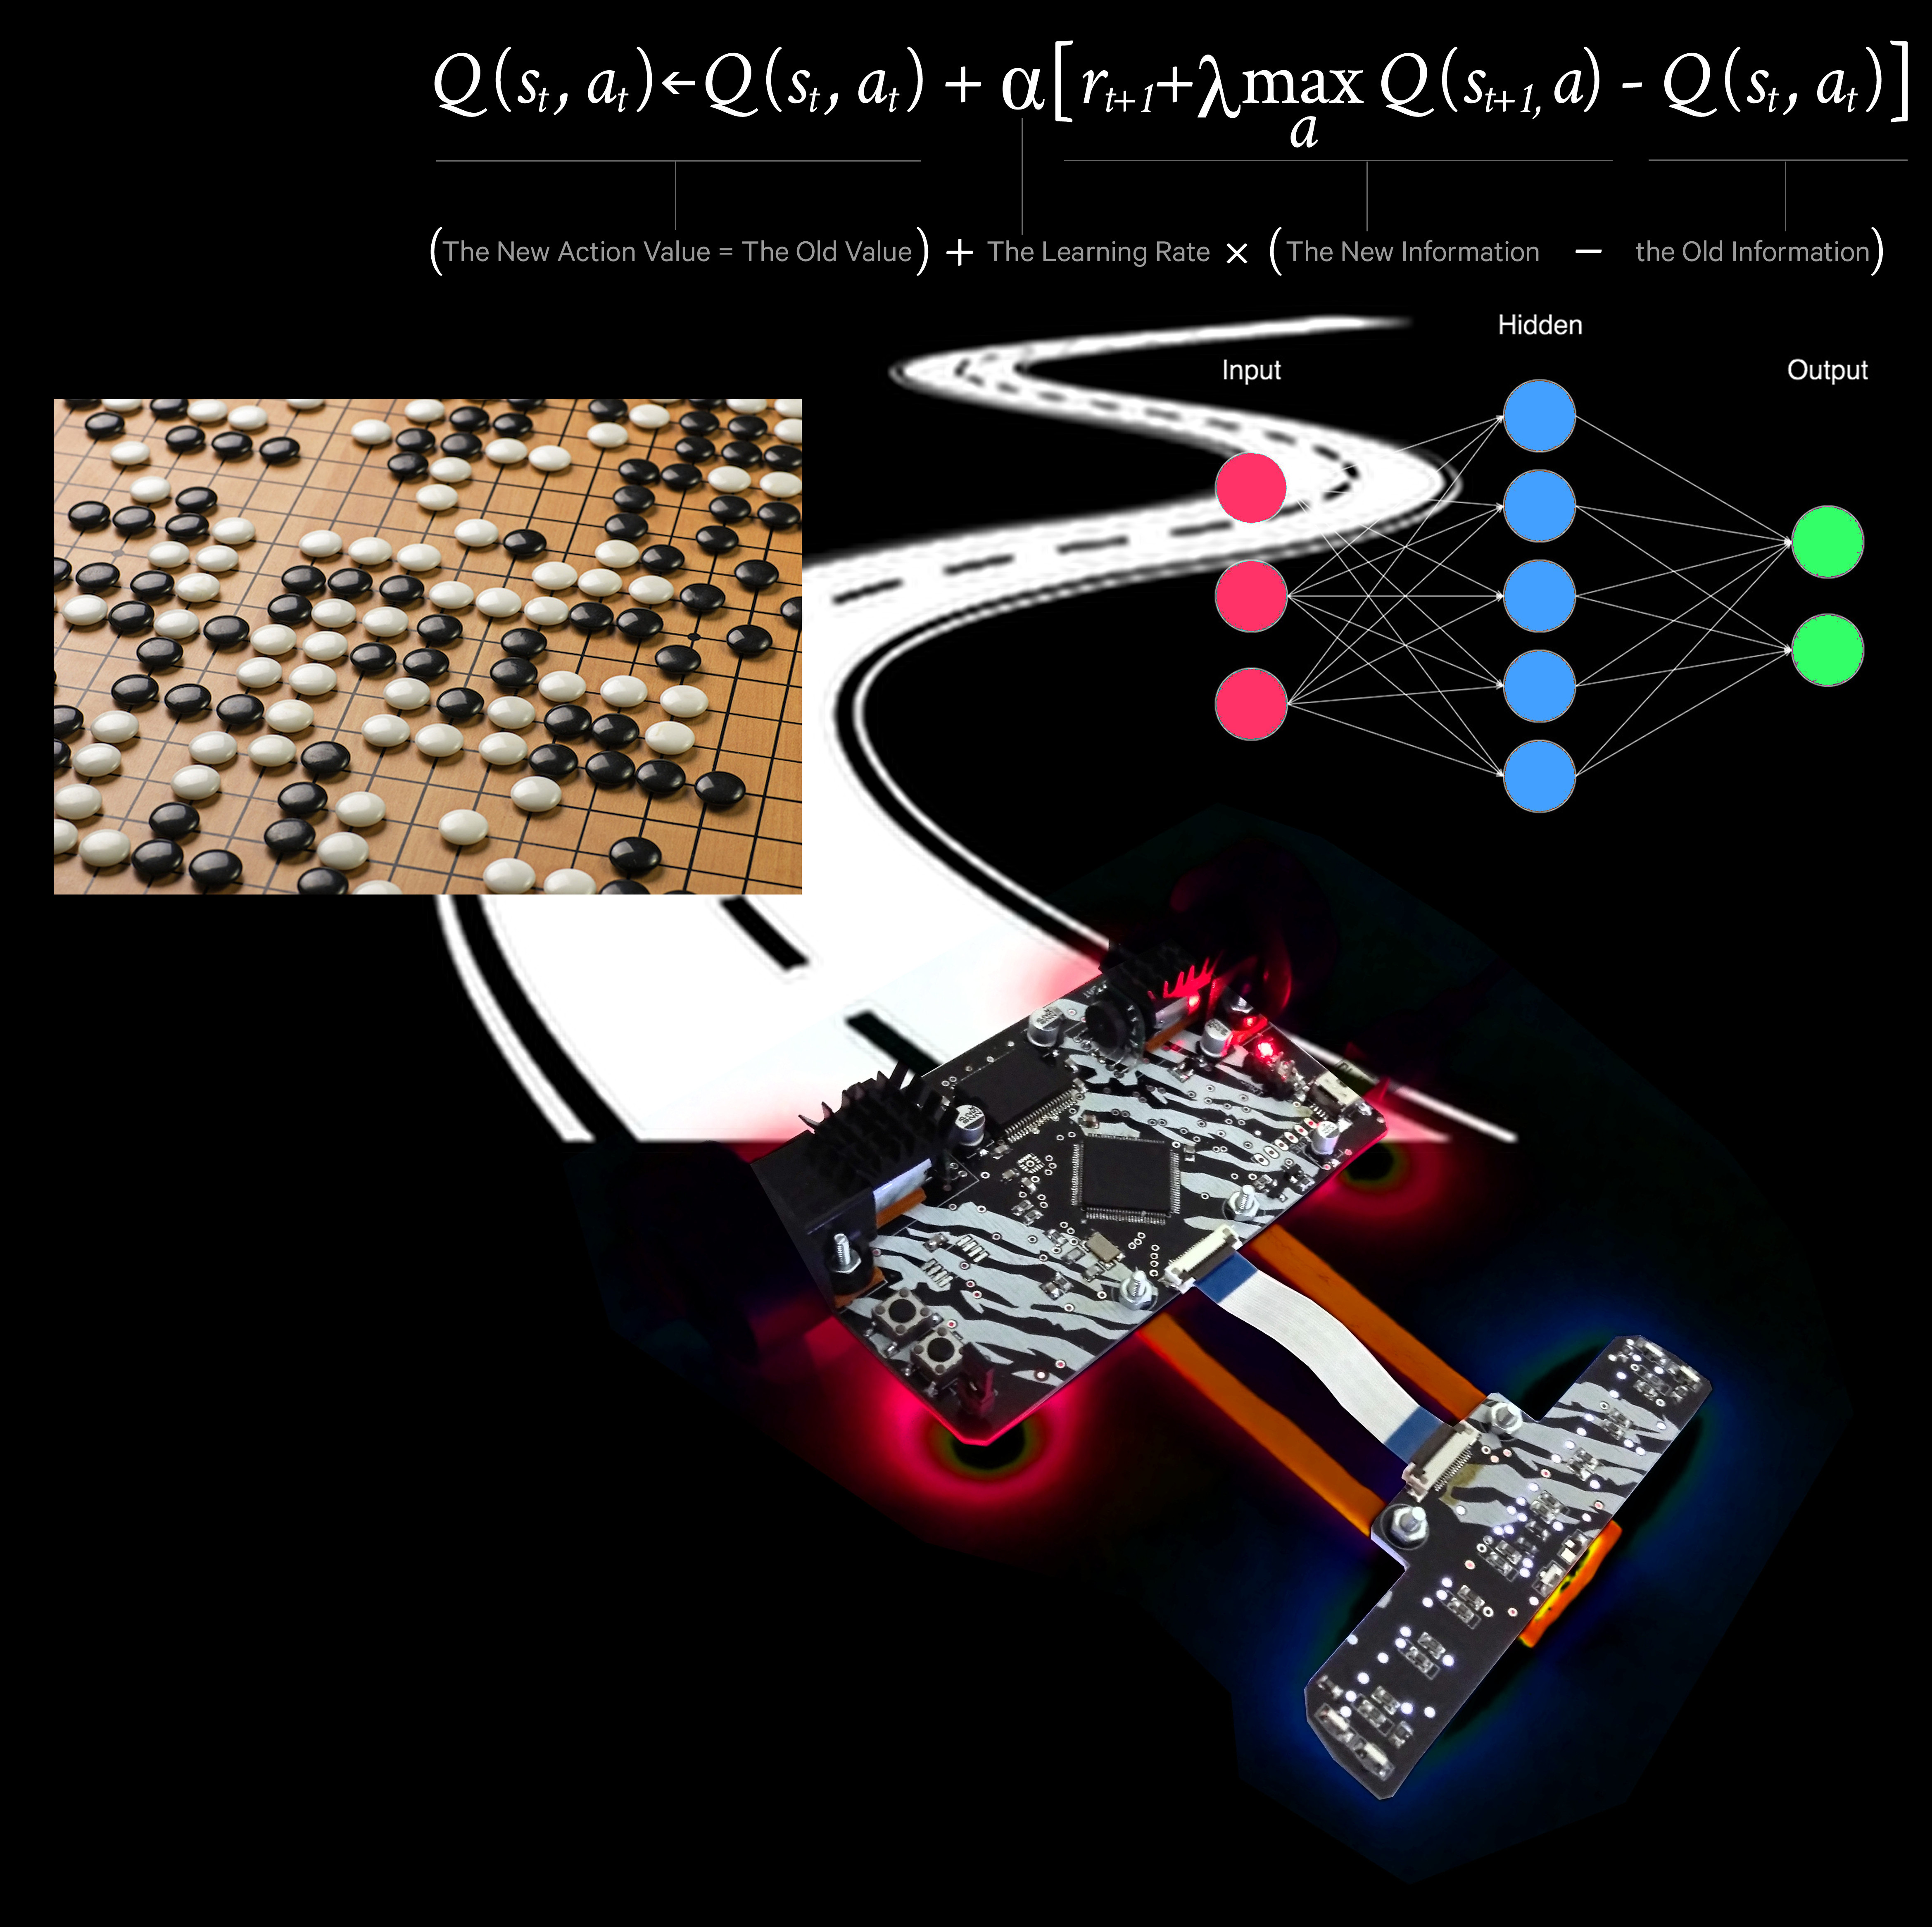
\includegraphics[width=5.05in]{../../pictures/rl_square.jpg}}

        \hfil}\vfil}
    }
    \begin{frame}

    %\titlepage


    \centering
     \colorbox{black}
     {
        \begin{minipage}{7cm}
           {\LARGE \color{white} \bf Reinforcement learning} \\
           {\LARGE \color{white} Michal CHOVANEC, PhD} \\
       \end{minipage}
     }


    \end{frame}
}



\begin{frame}{\bf Reinforcement learning}

\begin{itemize}
  \item learn from punishment and rewards
  \item learn to play a game with unknown rules
\end{itemize}

\begin{columns}
\begin{column}{0.5\textwidth}

  \begin{figure}
    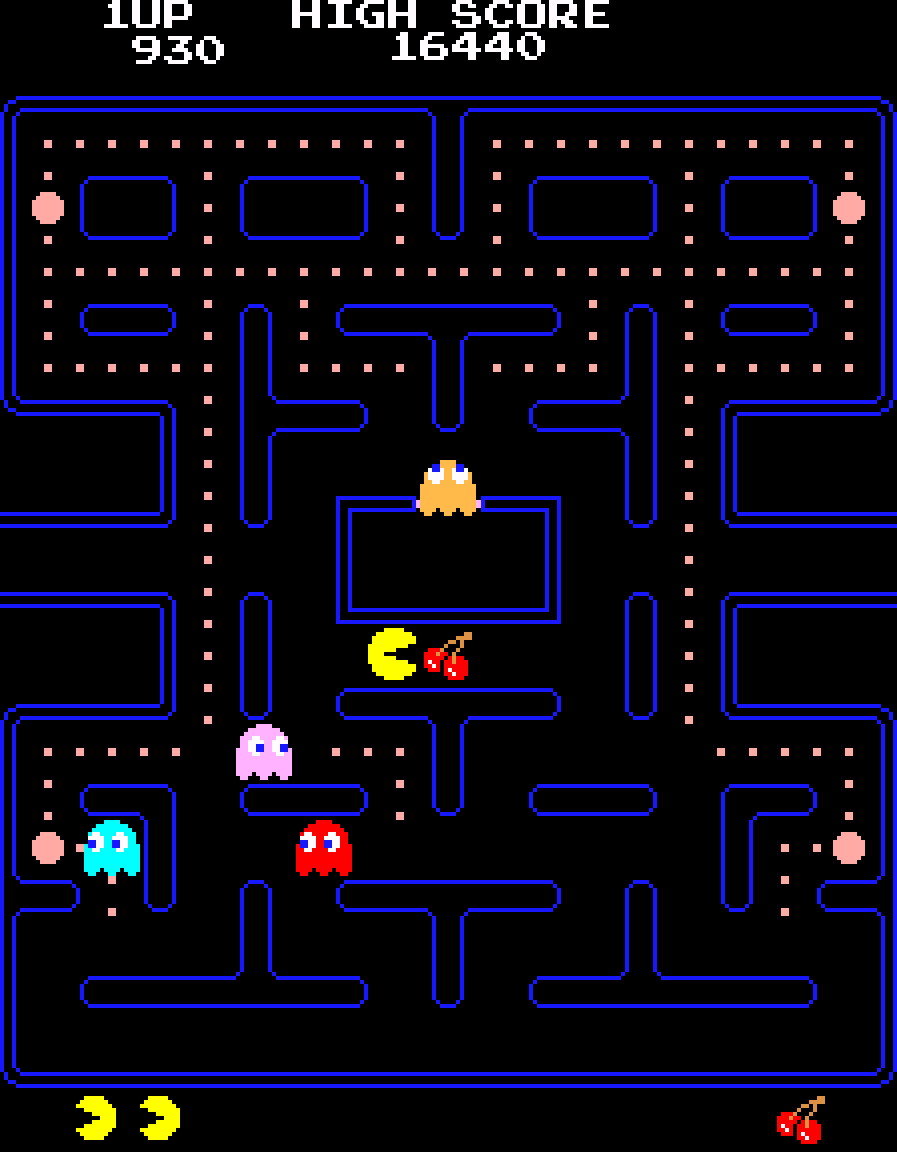
\includegraphics[scale=0.5]{../../pictures/pacman.jpg}
  \end{figure}

\end{column}
\begin{column}{0.5\textwidth}  %%<--- here

  \begin{figure}
  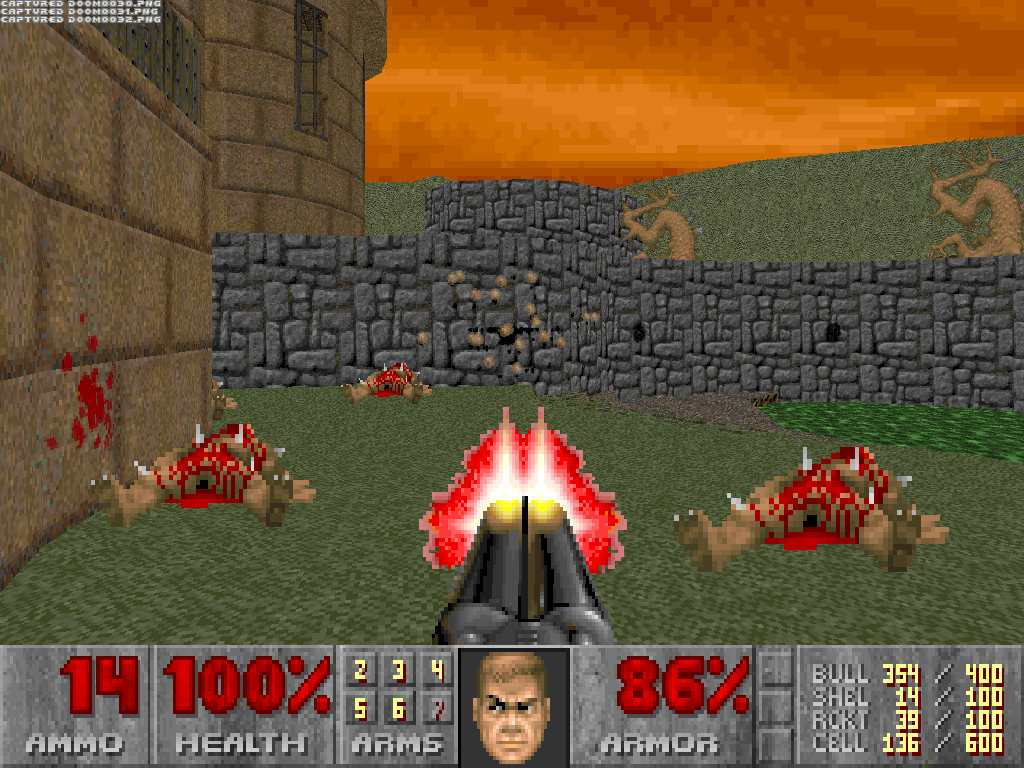
\includegraphics[scale=0.15]{../../pictures/doom.jpg}
  \end{figure}

\end{column}
\end{columns}

\vspace{-40pt}
\begin{figure}
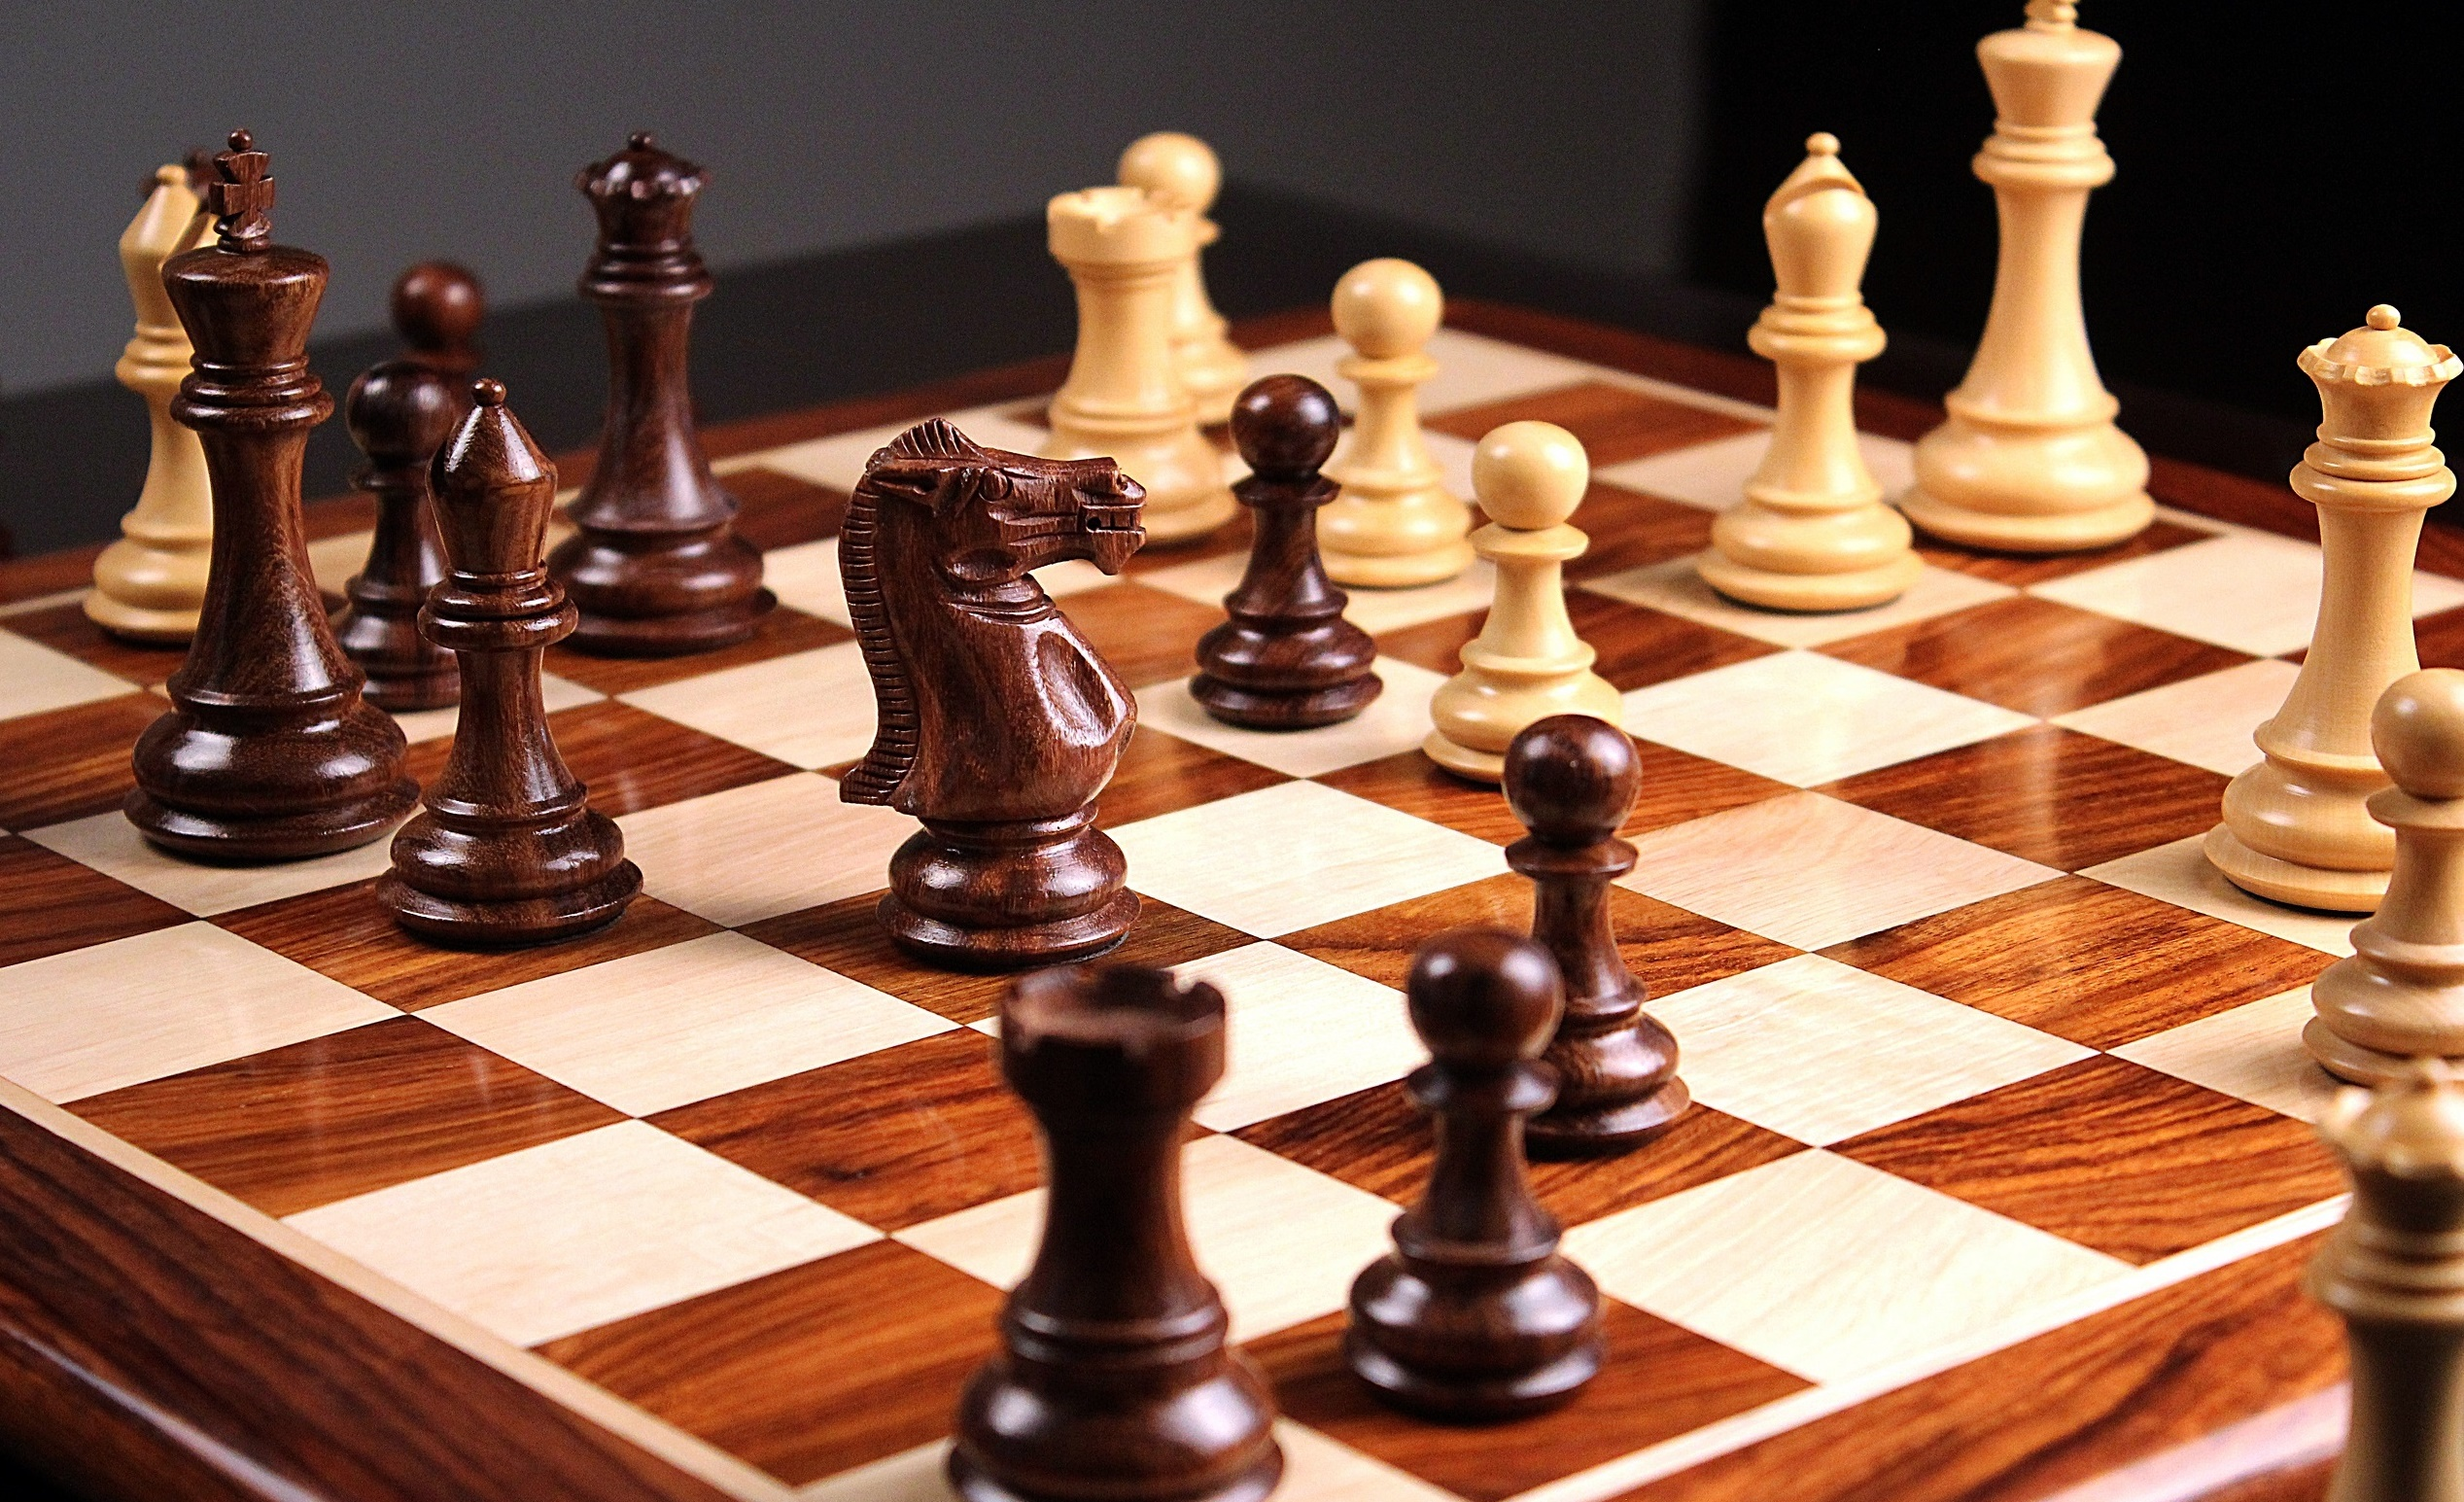
\includegraphics[scale=0.05]{../../pictures/chess.jpg}
\end{figure}

\end{frame}




\begin{frame}{\bf Reinforcement learning}

\begin{itemize}
  \item obtain {\bf state}
  \item choose {\bf action}
  \item {\bf execute} action
  \item obtain {\bf reward}
  \item learn from {\bf experiences}
\end{itemize}

  \begin{figure}
    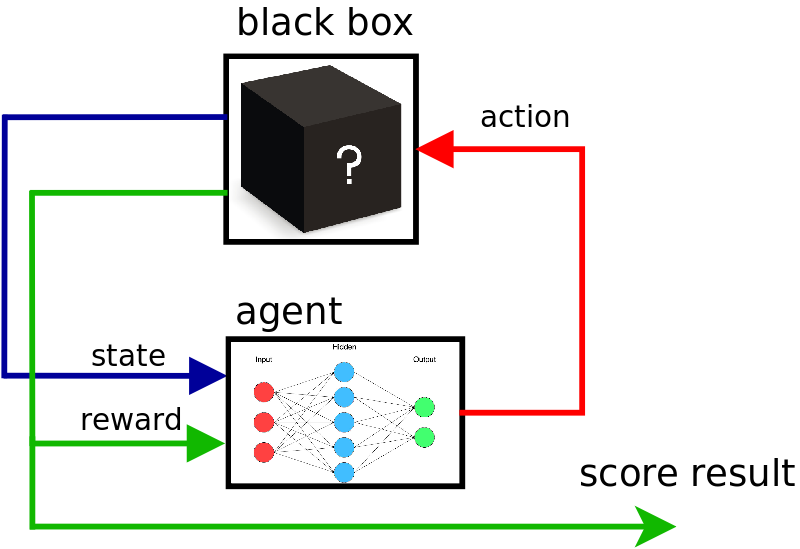
\includegraphics[scale=0.3]{../../diagrams/rl_mechanism.png}
  \end{figure}

\end{frame}



\begin{frame}{\bf Q learning}

\begin{align*}
Q'(s, a) = R + \gamma \max \limits_{\alpha'} Q(s', \alpha')
\end{align*}

where \\
$s$ is state \\
$a$ is action \\
$s'$ is next state \\
$a'$ is best action in next state \\
$R(s, a)$ is reward \\
$\gamma \in \langle 0, 1 \rangle$ is discount factor \\

\end{frame}





\begin{frame}{\bf Deep Q network - DQN}

\begin{align*}
\hat{Q}(s, a; w)&= R + \gamma \max \limits_{\alpha} \hat{Q}(s', \alpha; w), \\
\hat{Q}(s, a; w)&= R + \gamma \max \limits_{\alpha} \hat{Q}(s', \alpha; w')
\end{align*}


\end{frame}


\begin{frame}{\bf Dueling deep Q network - DDQN}

\begin{align*}
\hat{Q}(s, a; w)&= \hat{V}(s, a; w) + \hat{A}(s, a; w)
\end{align*}

\begin{align*}
\hat{Q}(s, a; w)&= R + \gamma \max \limits_{\alpha} \hat{Q}(s', \alpha; w), \\
\hat{Q}(s, a; w)&= R + \gamma \max \limits_{\alpha} \hat{Q}(s', \alpha; w')
\end{align*}


\end{frame}





\begin{frame}{\bf Usefull links}

{\tiny
  \begin{thebibliography}{9}
    \bibitem {}Andrej Karpathy : Pong from pixels \\ \url{http://karpathy.github.io/2016/05/31/rl/}
    \bibitem {}Richard S. Sutton : Reinforcement Learning: An Introduction \\ \url{https://www.amazon.com/Reinforcement-Learning-Introduction-Adaptive-Computation/dp/0262193981}
    \bibitem {}Maxim Lapan : Deep reinforcement learning \\ \url{https://www.amazon.com/Practical-Reinforcement-Learning-Maxim-Lapan/dp/1788834240}
    \bibitem {}Mohit Sewak : Practical Convolutional Neural \\ Networks \url{https://www.amazon.com/Practical-Convolutional-Neural-Networks-Implement/dp/1788392302}
    \bibitem {}CHRISTOPHER  J.C.H. WATKINS : Q-learning \\ \url{http://www.gatsby.ucl.ac.uk/~dayan/papers/cjch.pdf}
    \bibitem {}Densely Connected Convolutional Networks \\ \url{https://arxiv.org/pdf/1608.06993.pdf}
    \bibitem {}Mastering the Game of Go without Human Knowledge \\ \url{https://deepmind.com/documents/119/agz_unformatted\_nature.pdf}
  \end{thebibliography}
}

\end{frame}


\begin{frame}{\bf Q\&A}

\begin{figure}
  
\includegraphics[scale=0.25]{../../pictures/me.jpg}
\end{figure}

\centering {
michal chovanec (michal.nand@gmail.com)
\url{www.youtube.com/channel/UCzVvP2ou8v3afNiVrPAHQGg}
}

\centering {
github
\url{https://github.com/michalnand}
}

\end{frame}


\end{document}
